\documentclass{article}
\usepackage[utf8]{inputenc}
\usepackage{tikz}
\usetikzlibrary{shapes.geometric}
\usepackage{standalone}
\usepackage{amsmath}
\usepackage{amsfonts}
\usepackage[a4paper,margin=2.5cm]{geometry}


\newcommand{\red}[1]{{\color{red}{#1}}}

\newcommand{\bA}{\mathbf{A}}
\newcommand{\bB}{\mathbf{B}}
\newcommand{\bb}{\mathbf{b}}
\newcommand{\E}{\mathbb{E}}
\newcommand{\Norm}{\mathcal{N}}
\newcommand{\Loss}{\mathcal{L}}
\newcommand{\R}{\mathbb{R}}
\newcommand{\bt}{\mathbf{t}}
\newcommand{\bU}{\mathbb{U}}
\newcommand{\bu}{\mathbf{u}}
\newcommand{\bw}{\mathbf{w}}
\newcommand{\bX}{\mathbf{X}}
\newcommand{\bx}{\mathbf{x}}
\newcommand{\by}{\mathbf{y}}
\newcommand{\bZ}{\mathbf{Z}}
\newcommand{\bz}{\mathbf{z}}

\newcommand{\eq}{=}
\newcommand{\parfrac}[2]{\frac{\partial #1}{\partial#2}}




\title{Working title: Causal Effect Inference with Normalizing Flows}
\author{Micha de Groot}
\date{August 2019}

\begin{document}
\maketitle


\section{Introduction} 
Various scientific disciplines try to find patters in data. The patters that are usually uncovered are correlations between certain variables and features in the observations. In may fields this is a powerful tool that has resulted in tremendous scientific progress. Especially in AI we can perform a abundance of tasks, such as classification of images, translation of text or even the generation of new music. % citation needed
But what most scientists actually want to find out is what the causal relations of things are and correlations are merely a way to indicate a possible causal relation. The inherent problem with correlation-based methods is of course that they can never find causal relations.

Every class in statistics starts with the phrase: "Correlation is not causation." This mantra tells us that we should never interpret a correlation between a variable $A$ and variable $B$ as $A$ causes $B$. This is very much true, but sometimes we do like to know: does $A$ cause $B$? To answer such questions we need causal inference. 

Disciplines such as medicine approach this problem through double-blind studies, in which the only difference between groups is whether or not they received a treatment, meaning that any difference between the two trial groups must have been caused by the treatment. Unfortunately the vast majority of problems can only be viewed through observational studies in which there usually is (unobserved) confounding between a variable $A$ and a variable $B$. Isolating the causal effect we are interested in from background variables can be a difficult task, as decades in statistical research has shown.

Fortunately the work by Pearl et al.\cite{pearl2009causal} \cite{pearl1995causal} has yielded a framework in which these causal effects can be modelled in terms of probability densities and in which it is theoretically possible to isolate a direct causal effect of a variable on another variable if there are one ore more unobserved confounding variables. This has led to an abundance of scientific research on how to properly measure and analyse causal effects in the past two decades(citation needed), especially focusing on how to leverage the ever-increasing amount of data that is available to us. 


%Measuring the causal effect of an action or treatment on certain parts of the world and the people in it is a question that form the cornerstone of most sciences\footnote{\label{note:citation}Citation needed}.

The area of generative modelling within AI has shown a series of successes in recent years. This area tries to learn the structure within data and uncover the process with which it was generated. Such models have the power to <> the latent variables of the data. That ability is invaluable if we want to want to model latent confounders and be able to estimate causal effects. Using machine learning techniques also indicates that having mode data is useful for making more accurate predictions. %TODO



\section{Background}

\subsection{causal inference, interventions and do-calculus}
%The dominant research in artificial intelligence is all data-driven and broadly speaking looking for patterns in said data. The patters that most common AI models uncover are correlations between certain features in the data. In may problems this is a powerful tool that can perform a abundance of tasks, such as classification of images, translation of text or even the generation of new music. However, there is an inherent limit to models that can only uncover correlations: they can't find causal relation. Every class in statistics starts with the phrase: "Correlation is not causation." This mantra tells us that we should never interpret a correlation between a variable $A$ and variable $B$ as $A$ causes $B$. This is very much true, but sometimes we do like to know: does $A$ cause $B$? To answer such questions we need causal inference. 

In the causal inference framework, devised largely by Judea Pearl\cite{pearl1995causal} \cite{pearl2009causal}, we go beyond correlations by modelling the direction of cause and effect as well. This is done by modelling variables or events, and their relations as Directed Acyclic Graphs (DAG); The state of each variable is defined as a function of all its parents in such a graph, called structural equations.

An example of several DAGs is given in Figure \ref{fig:graph_correlations_A_B}. Combined with the structural equations for each edge in the graph, these form a Structural Causal Model. If the true graphs and functions would be known, we would precisely know all causal effects. Of course such a strong claim is followed by the observation that the space of possible DAGs grows super exponentially with the number of vertices; That number grows to 29281 possible graphs when there are five vertices, and to 1138779265 possible graphs when there are seven vertices \cite{robinson1977counting}. Some methods have been developed to address this problem, but that goes beyond the scope of this thesis. Instead we focus on the estimation of the structural equations for problem where we know or have good reasons to assume a certain graph structure.



\begin{figure}
    \centering
    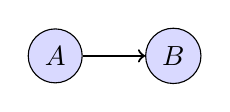
\begin{tikzpicture}
        \node[draw=black, circle, fill=blue!15!white] (a) at (0, 0) {$A$};
        \node[draw=black, circle, fill=blue!15!white] (b)at (1.5, 0) {$B$};
        \draw[->, thick] (a) -- (b);
    \end{tikzpicture}
    \qquad
    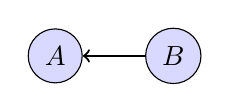
\begin{tikzpicture}
        \node[draw=black, circle, fill=blue!15!white] (a) at (0, 0) {$A$};
        \node[draw=black, circle, fill=blue!15!white] (b)at (1.5, 0) {$B$};
        \draw[->, thick] (b) -- (a);
    \end{tikzpicture}
    \qquad
    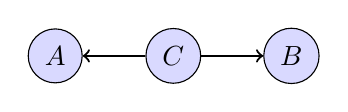
\begin{tikzpicture}
        \node[draw=black, circle, fill=blue!15!white] (a) at (0, 0) {$A$};
        \node[draw=black, circle, fill=blue!15!white] (b) at (3, 0) {$B$};
        \node[draw=black, circle, fill=blue!15!white] (c) at (1.5, 0) {$C$};
        \draw[->, thick] (c) -- (b);
        \draw[->, thick] (c) -- (a);
    \end{tikzpicture}
    \caption{Three possible DAGs for when $A$ and $B$ are correlated. On the left hand side $A$ causes $B$, in the middle $B$ causes $A$ and on the right hand side both $A$ and $B$ are caused by a third variable $C$.}
    \label{fig:graph_correlations_A_B}
\end{figure}


The reason we want to estimate these functions is to answer causal questions. Although some cause and effect relations might seem deterministic, they are usually framed in a statistical fashion. This makes it possible to relate it to statistics and correlations, and in some cases even rephrase a causal question as a mere statistical one. The most important component in that regard is the \textit{do}-operator, see Equation \ref{equation:do_operation}. This equation tells us the probability of $A$ if we were to \textit{set} $B$ to a specific value; This is the causal effect from $B$ on $A$ in a probabilistic framing. The $pa_{B}$ is this equation indicates the set of all parents of $B$ in the causal graph, and if they are also parents of $A$ they are called confounders of $A$ and $B$. This immediately shows that we have to have knowledge of the causal graph to quantify a causal effect. For clarity  Equation \ref{equation:do_operation} also shows the conditional probability of $A$ given $B$ if we were to factor out the other parents of $A$. These two equations reduce to the same in certain cases, such as when $A$ has no parents, or when $B$ is the only parent of $A$. 
%Convince yourself that this is the case by looking back at Figure \ref{fig:graph_correlations_A_B}.

\begin{align}\label{equation:do_operation}
    p(A | do(B)) &= \int_{pa_B} p(A | B, pa_{B}) p(pa_{B}) \text{d} pa_B\\
    p(A | B) &= \int_{pa_B} p(A | B, pa_{B}) p(pa_{B}|B) \text{d} pa_B
\end{align}

Now the question arises: why is causal inference then perceived to be such a difficult problem if we can just slightly adjust an existing equation for computing conditional probabilities? This is because we either don't know the structure of the graph at all or if we can't observe certain confounders in the graph, called \textit{latent} confounders. But, given a graph structure, there are ways to estimate the causal effects, even when some variables are unobserved. The rest of this section will cover existing work on causal inference and how we evaluate such estimations.

%If we don't know the graph we have to resort to causal discovery, which is beyond the scope of this research. If we do know the structure of the graph, or have strong indications to assume a certain structure, we can resort to methods to estimate the structural equations, even if not all variables are observed. The rest of this section will cover the existing work on causal inference in the case where there is a latent confounder.


% After that we will at some point talk about do-calculus and how you can measure a causal effect if you know the graph. Backdoor adjustment. Something about assuming a graph structure.

% Existing work on causal inference that doesn't use deep learning


\subsubsection*{Approximating the latent confounder through a proxy variable}
In lost of cases the true confounder of the variables of interest is unknown, but a proxy variable might be available\cite{kuroki2014measurement}\cite{miao2018identifying}. For instance in the case where we want to know the causal effect of regular exercise on health. In such a case it is plausible to assume that there are some intrinsic features of a person that makes him both more inclined to exercises himself and that also has other, maybe beneficial, effects on health. In other words a latent confounder. Such characteristics are typically not known, but there might be features that we can measure, such as blood pressure, BMI or age. These are also partially caused by these intrinsic features. In that case we have a causal graph as in Figure \ref{fig:causal_graph_with_proxy}, where there is a proxy variable that tells us something about our latent confounder.

There are multiple graphs that represent a scenario with proxy variables. Miao et al. describe six possibilities, with graphs that contain up to five nodes, two of which are proxies. One or both of these proxies can also be a cause of the treatment and outcome respectively. Such cases give a more powerful proxy, as we can then observe more direct effects in the graph. The scenario where the proxy gives the least information is the one shown in Figure \ref{fig:causal_graph_with_proxy}, and that is the one we will focus on. Because if we can infer causal relations in such a graph then we can also do it in all other graphs with proxies.

%TODO. Done for now.

\begin{figure}[b]
    \centering
    \includestandalone{Figures/causal_graph_one_proxy_one_confounder}
    \caption{Causal graph with one proxy variable. $\bt$ is the variable we intervene on; $\by$ is the outcome; $\bZ$ is the latent confounder; and $\bX$ is the observed proxy variable.}
    \label{fig:causal_graph_with_proxy}
\end{figure}


\subsubsection*{Metrics in causal inference}
In most causal inference scenarios there is a binary treatment or cause variable and one would like to know what the effect of that variable on an outcome variable is. This is phrased as the difference in outcome when intervening on the treatment and not intervening on the treatment: $$ATE := \E[\by|do(\bt=1)] - \E[\by | do(\bt=0)]$$This is called the Average Treatment Effect(ATE) \cite{shalit2017estimating}\cite{johansson2016learning}\cite{kunzel2019metalearners}. To calculate it exactly we would need to integrate over the latent confounders:
$$
    p(\by|do(\bt=1)) = \int_\bZ p(\by|\bt=1, \bZ) p(\bZ) d \bZ    
$$
The ATE is an effect measured over the entire dataset or population. It is interesting to know in cases where one has to decide on a general policy. In individual cases such a population is less meaningful and we want to look at the potential effect on individual people \cite{shalit2017estimating}\cite{johansson2016learning}\cite{kunzel2019metalearners}. For that there is the Individual Treatment Effect(ITE) or Conditional Average Treatment Effect (CATE): $$ITE := \E[\by|do(\bt=1)|\bX=x] - \E[\by | do(\bt=0), \bX=x]$$ Here we condition on a specific set of \textit{proxy} features to look a the effect on a specific sub-population. 
\begin{equation}\label{equation:intervention_with_proxy}
    \begin{split}
    p(\by | \bX=x, do(\bt=1)) &= \int_\bZ p(\by | \bX=x, do(\bt=1, \bZ)) p(\bZ | \bX=x, do(\bt = 1)) d\bZ \\
                            &= \int_\bZ p(\by | \bX=x, \bt = 1, \bZ) p(\bZ | \bX=x) d\bZ
    \end{split}
\end{equation}

\noindent
Both of these integrals, of the ATE and ITE, are in general not tractable, especially if $\bZ$ is unobserved. To circumvent that methods to approximate the posterior of $\bZ$ are needed.

% \subsubsection*{Distinguishing cause from effect using observational data: methods and benchmarks}
% --Book (chapter)\cite{mooij2016distinguishing}, quite long, will look for useful info--

% Causal discovery in the bivariate case has been mostly based on the difference in complexity of the factorisation of the joint distribution $p(X,Y)$. If $p(X)p(Y|X)$ consists of two simpler distributions than $p(Y)p(X|Y)$ then it is likely that $X$ is a cause of $Y$ instead of the other way around. The chapter discusses several extensive benchmarks for these types of tests.

% Another definition for "$X$ is a cause of $Y$" is that $p(Y|do(X=x)) \neq p(Y|do(X=x'))$
% %TODO



\subsection{Deep learning and Generative modelling}

\subsubsection*{Autoencoding Variational Bayes}
The problem of finding the posterior distribution of the latent variable of data is a problem that has been approached with different methods. Variational Inference is one of such methods, which has become very popular through the Variational Autoencoder(VAE) \cite{kingma2013auto}. The VAE is a framework that uses the principle of a variational distribution to approximate the posterior distribution. Because of the positioning of the VAE within the deep learning it was able to distinguish itself from other variational inference methods. 

The loss that a VAE optimises is called the Evidence Lower Bound (ELBO) or negative free energy. The name comes from the  fact that it is lower bound for the log likelihood $\log p_\theta(\bx)$, see Equation \ref{equation:negative_free_energy}. By using neural networks to parameterise the variational distribution and the likelihood, and the reparameterisation trick, it is possible to learn the variational distribution and the data likelihood, the two parts of the ELBO, through gradient descent methods.

\begin{equation}\label{equation:negative_free_energy}
    \begin{split}
    \log p_\theta(\bx) &= \log \int p_\theta(\bx | \bz) p(\bz) d\bz\\
    &= \log \int \frac{q_\phi(\bz|\bx)}{q_\phi(\bz|\bx)} p_\theta(\bx | \bz) p(\bz) d\bz\\
    &\geq -\mathbb{D}_{KL}[q_\phi(\bz|\bx) || p(\bz)] + \mathbb{E}_q[\log p_\theta(\bx|\bz)] = -\mathcal{F}(\bx)
    \end{split}    
\end{equation}
    

Although the VAE has been used successfully for variational inference, it does have its limits. A requirement for a VAE is that the variational distribution is a parameterised distribution that is chosen beforehand, usually a Gaussian with diagonal covariance. This of course limits the model in capturing more complex posterior distributions. Another disadvantage is that the likelihood tends to converge to a per-feature mean. This means that in datasets where individual features are either multimodal or are far from the mean, given a specific value of the latent value, the likelihood is fitted poorly on the data. This is apparent in image-based datasets. The images sampled from the model tend to be very blurry and lack sharp edges.

\subsubsection*{Variational Inference with Normalising Flows}
A normalising flows is a type of model that is capable of variational inference. Is is able to learn flexible, arbitrarily complex and scalable approximate posterior distributions. The main advantage it has over the VAE is that the approximation of the posterior is not limited to parameterised distributions. The idea is to start with a simple initial density that is parameterised, and transforming that into an arbitrary complex distribution by applying a series of invertible transformations. The final probability density is defined by applying the change of variable formula to the density of the original simple distribution, as shown in equation \ref{equation:change_of_variable}. The only requirement of the invertible mapping is that its Jacobian has to be efficiently computed, as it has to be evaluated many times, both during training and testing.

\begin{align}\label{equation:change_of_variable}
    \bz_K &= f_K \circ ... \circ f_1 (\bz_0)\\
    p(\bz_K) &= p(\bz_0) \prod\limits_{k=1}^K \left|\det \parfrac{f_k}{\bz_{k-1}} \right|^{-1}\\
    \log p(\bz_K) &= \log p(\bz_0) - \sum\limits_{k=1}^K \log \left|\det \parfrac{f_k}{\bz_{k-1}} \right|
\end{align}

\noindent
This can be applied by augmenting the VAE by taking the original, relatively simple, variational distribution and passing that through a series of such function, thereby reaching the more complex approximation of the posterior. The ELBO then has to be extended by substituting a part of it with the change of variable equation stated above. This is show in equation \ref{equation:negative_free_energy_with_flow}. Note here that this yields us an objective very similar to the original ELBO with just the log determinant Jacobian added to it.

\begin{equation}\label{equation:negative_free_energy_with_flow}
    \begin{split}
    -\mathcal{F}(\bx) &= -D_{KL}[q_\phi(\bz|\bx) || p(\bz)] + \E_{q_\phi(\bz|\bx)}[\ln p_\theta(\bx|\bz)]\\
    &= \E_{q_\phi(\bz|\bx)}[-\ln q_\phi(\bz|\bx) + \ln p(\bz) + \ln p_\theta(\bx|\bz)]\\
    &= \E_{q_0(z_0)}[-\ln q_0(\bz_K) + \ln p(\bz) + \ln p_\theta(\bx|\bz_K)]\\
    &= \E_{q_0(z_0)}[-\ln q_0(\bz_0) + \sum\limits^K_{k=1}\ln \left|\text{det} \parfrac{f_k}{\bz_{k-1}} \right| + \ln p(\bz) + \ln p_\theta(\bx|\bz_K)]\\
    &= -D_{KL}[q_0(\bz_0|\bx) || p(\bz)]+   \E_{q_0(z_0)}[\sum\limits^K_{k=1}\ln \left|\text{det} \parfrac{f_k}{\bz_{k-1}} \right| + \ln p_\theta(\bx|\bz_K)]\\
    \end{split}
\end{equation}

\noindent
Rezende and Mohamed also propose two possible functions that fulfil the requirement of having a tractable log determinant Jacobian, called the Planar Flow and Radial Flow. Both these functions consist of a residual connection to which a simple transformation to the input is added. Even though both of these flow types apply a small change per function, they can reach a complex transformation by stacking enough of them.

%The negative free energy function $\mathcal{F}$ is also known as the Evidence Lower Bound(ELBO). The novelty of normalising flows lies in how the approximate posterior $q_\phi(\bz|\bx)$ is defined.  


\subsubsection*{Density estimation using Real-NVP}
The Normalising Flows paradigm has given rise to several other models, one of which is the Real-NVP \cite{dinh2016density}. The Real-NVP also work by chaining a series of invertible functions that have a tractable log determinant Jacobian. Dinh et al. have achieved this by designing so-called coupling layers. These coupling layers each apply a translation and scaling to a part of the current input. The other half is copied, see Figure \ref{fig:real_nvp_graph}. By changing which part is copied and which is altered every coupling layer you can reach complex transformations to your whole vector. The scaling and translation of one half of the vector are determined by neural networks that each take the other half of the vector as input. Fortunately the log determinant Jacobian of the coupling layer does not require the determinant of the neural networks, meaning those networks can be arbitrarily complex.

\begin{figure}
    \centering
    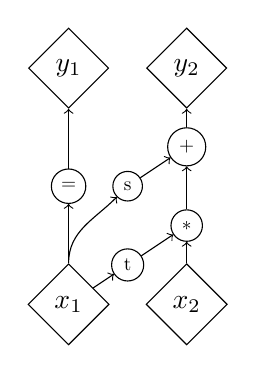
\begin{tikzpicture}
        \node[draw, diamond] (y1) at (0,0) {$y_1$};
        \node[draw, diamond] (y2) at (1.5,0) {$y_2$};
        \node[draw, diamond] (x1) at (0,-3) {$x_1$};
        \node[draw, diamond] (x2) at (1.5, -3) {$x_2$};
        \node[draw, circle, scale=0.7] (+) at (1.5, -1) {$+$};
        \node[draw, circle, scale=0.7] (=) at (0, -1.5) {$=$};
        \node[draw, circle, scale=0.7] (*) at (1.5, -2) {$*$};
        \node[draw, circle, scale=0.7] (s) at (0.75, -1.5) {s};
        \node[draw, circle, scale=0.7] (t) at (0.75, -2.5) {t};
        
        \draw[->] (x1) -- (=);
        \draw[->] (=) -- (y1);
        \draw[->] (x1) edge[out=90, in=225] (s);
        \draw[->] (x1) -- (t);
        \draw[->] (s) -- (+);
        \draw[->] (t) -- (*);
        \draw[->] (x2) -- (*);
        \draw[->] (*) -- (+);
        \draw[->] (+) -- (y2);
    \end{tikzpicture}
    \qquad
    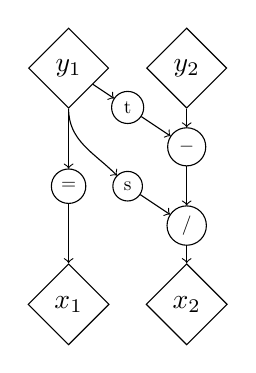
\begin{tikzpicture}
        \node[draw, diamond] (y1) at (0,0) {$y_1$};
        \node[draw, diamond] (y2) at (1.5,0) {$y_2$};
        \node[draw, diamond] (x1) at (0,-3) {$x_1$};
        \node[draw, diamond] (x2) at (1.5, -3) {$x_2$};
        \node[draw, circle, scale=0.7] (-) at (1.5, -1) {$-$};
        \node[draw, circle, scale=0.7] (=) at (0, -1.5) {$=$};
        \node[draw, circle, scale=0.7] (/) at (1.5, -2) {$/$};
        \node[draw, circle, scale=0.7] (s) at (0.75, -1.5) {s};
        \node[draw, circle, scale=0.7] (t) at (0.75, -0.5) {t};
        
        \draw[->] (y1) -- (=);
        \draw[->] (=) -- (x1);
        \draw[->] (y1) edge[out=270, in=135] (s);
        \draw[->] (y1) -- (t);
        \draw[->] (s) -- (/);
        \draw[->] (t) -- (-);
        \draw[->] (y2) -- (-);
        \draw[->] (-) -- (/);
        \draw[->] (/) -- (x2);
    \end{tikzpicture}
    \caption{Coupling layer of the Real NVP and its inverse}
    \label{fig:real_nvp_graph}
\end{figure}

\subsubsection*{Analyzing Inverse Problems with Invertible Neural Networks}
The invertbility of flow-based models makes them suitable for recovering posterior information of complex physical systems. This has been proposed by Ardizzone et al. \cite{ardizzone2018analyzing} in the form of Invertible Neural Networks. Given some process $\bx \rightarrow \by$ with observed $\by$ and unobserved $\bx$ oe would like to know how to recover $\bx$ for a ceartain $\by$. This is done by using an approach based on the Real-NVP\cite{dinh2016density} model. Since the forward process has inherent information loss, a latent variable $\bz$ is introduced that captures the information in $\bx$ that is not contained in $\by$, turning the process into $f(\bx) = [\by, \bz]$  and $\bx = f^{-1}(\by, \bz) = g(\by, \bz)$. Because of the nature of Normalising-Flow models, $g(\by, \bz)$ does not have to be modelled separately. The density $p(\bz)$ is shaped as a Gaussian. 

This differs from the causal graph in Figure \ref{fig:causal_graph} because both $\bx$ and $\bz$ are unobserved. Though the INN approach might still be useful if we were to recover $\bZ$ from a given $\bX$. I think this would be an approximation for $p(\bZ | \bX)$, which could then be used to approximate equation \ref{equation:intervention}. % Veranderen


\subsubsection*{Sylvester Normalising Flows for Variational Inference}
Another flow-based model is the Sylvester Normalising Flow\cite{berg2018sylvester}. This is a direct adaptation of the planar flow designed by Rezende and Mohamed. The planar flow function consist of a residual connection and a linear layer with a bottleneck of one dimension (and a non-linearity), see equation \ref{equation:planar_flow_sylvester_flow}. The reason for that is to have a closed form solution of the log determinant Jacobian. Van den Berg et al. came up with a version that does not require a bottleneck of one dimension, allowing the mappings to learn far more transformations.

\begin{align}\label{equation:planar_flow_sylvester_flow}
    f_{planar}(\bz) &= \bz + \bu h(\bw^T\bz + b)\\
    f_{sylvester}(\bz) &= \bz + \bA h(\bB\bz + \bb)
\end{align}

By making use of Sylvester's determinant identity and a QR-factorisation of matrices $\bA$ and $\bB$ in equation \ref{equation:planar_flow_sylvester_flow}, the transformation can be rewritten in such a way that it has a tractable Jacobian. The resulting matrices $Q$ and $R$ of the QR-factorisation do have to be kept orthogonal and triangular respectively. The paper by van den Berg et al. proposes several methods to do this during training.

\subsubsection*{Generative Adversarial Networks}
A Generative Adversarial Network (GAN) is another type of generative model\cite{goodfellow2014generative}. It differs from the model described above in several aspects. Firstly is doesn't model the posterior of the data in any way, it only models the prior and the likelihood. This is of course a downside of the model, but what it brings to the table is this: it uses adversarial learning to train the generator model. Instead of learning a mean squared error of each individual feature it concurrently trains another model, the discriminator model, that must label the generated image as either a real image from the dataset or a generated one. This classification error is the only thing that is backpropagated, both through the discriminator and the generator. The result of this is, in the case of an image dataset, a model that is capable of generating far sharper images than a VAE could. 

Because there is no posterior, a GAN can only generate completely random images. To allow some selection in what the model would generate, the conditional GAN was created \cite{mirza2014conditional}. A conditional GAN extend the GAN by conditioning the input of the generator not only on a random sample of the prior, but also on a conditional vector that represents a visual feature such as the person in the image having a moustache.  


\section{Research proposal}
The goal of this project is to see if it is possible to extent the work of Louizos et al. \cite{louizos2017causal} through the use of Normalising Flows. Louizos et al. have shown that variational inference can be used for causal inference. We now want to discover if we can improve of their VAE-based \cite{kingma2013auto} method with Normalising Flows \cite{rezende2016variational}\cite{berg2018sylvester}\cite{dinh2016density}. It has been shown that these models are capable of capturing more diverse and complex posterior distributions, which is needed in this research.

The first phase of the project directly extends the causal VAE to a causal VAE with Normalising Flow. We hypothesise that this works slightly better because the model can capture a more complex latent distribution. Though a limitation here is the complexity of the dataset and the causal effect that we want to model. The commonly used datasets in causal inference all have a binary, one-dimensional treatment or intervention variable and a one-dimensional scalar as outcome variable. The observed feature vectors are, by deep learning standards, very low dimensional. This all means that the potential modelling power that Normalising Flows possess probably won't reach their full potential. 

To display this full modelling power we are going to generalise the problem in the second phase. This will be split into different components and will likely be the core of the project.

\subsection{Directions in which we want to generalise the model}
Several steps that we want to take to generalise the problem
\begin{itemize}
    \item Step away from the assumption that the treatment is binary and one dimensional. We either make the treatment variable categorical or continuous. It also has to be higher dimensional, maybe in such a way that it can't be directly interpreted.
    \item Learn the intervention. In the original model all possible values of the intervention are known and seen during training. We want the model to learn the general concept of the intervention variable and being able to handle intervention samples that are (slightly) different from the ones in the training set.
    \item It is important in all these extensions that it shouldn't suffice to learn correlations between variables. It has to be the case that there is a causal effect with some form of latent confounding.
\end{itemize}


% \section{Learn the intervention}
% Don't assume that we (can) know all the values the intervention can take. Combine learning the outcome for a given intervention with learning what intervention will yield a <high> outcome.

% What is important to note here is that we are not necessarily looking for a model that takes good actions, but one that learns the causal effect of certain interventions. The novelty would be that the model could generalise to interventions that it hasn't seen before.

% \subsection{Construct a scenario where you really have to learn cause and effect}
% Some scenarios that could be predicted with our model could probably also be predicted with a model that learns correlations between the values of interventions, outcomes and features.

\subsection{New idea}
We need a problem where there is an effect of one variable $t$ on another variable $y$. We need to be able to observe both, but their dimensions might be entangled in some way. It could help if there is more information we can observe, $x$, that tells us more about a possible latent representation of the current sample/state. There \textbf{has} to be latent confounding between $t$, $y$ and $x$. Otherwise we could directly estimate covariates for $t$ and $y$ from $x$ without the need to model any latent variables/confounders. 

What is preferable is that the observed variables have a reasonable high dimensionality. For $t$ and $y$ that means at least three dimensions. For $x$ at least one hundred. An obvious direction for this would be to have images as our observed variables. Firstly this makes for a cooler presentation at the end, and secondly because there are no SOTA methods that can work with raw images that don't use any form of deep learning. This also makes the need for Normalising Flows more apparent because images have a complex distribution.

Now the question is: what can be the outcome variable in an image and what can be the intervention? We could have as input one image, $x$, an outcome image $y$ and an intervention $t$. Then it has to be the case that there always is a difference between $x$ and $y$ even if the intervention is zero. That would make it so that there is a difference between $x$ and $y$ that is partially caused by $t$ and partially caused by $z$, who's posterior we would estimate from $x$. It also has to be the case that $x$ is actually caused by $z$, but that can be arranged if we generate the images ourselves. 

%What would we actually measure in this setup? The modelling of the intervention or the modelling of the outcome or both?

\subsubsection*{Toy dataset idea}
We have an image $x$, that contains a shape, let's say a circle. It also contains an arrow (?) or other visual clue about what the intervention will be, or no clue if there is no intervention. The outcome $y$ is always different from $x$ to make sure there is confounding between the intervention and the outcome. But this difference is always independent of the intervention. Then the model has to reconstruct $x$ back from the latent space, learn what the intervention clue $t$ means and what the outcome $y$ will be after the intervention. The intervention can be that the shape has moved in the direction of the arrow for instance. The effect from $z$ on $y$ can also be a translation, or a linear transformation.

To actually know if the model has disentangled the shape from the intervention we can hold out something from the training set. We can either change the shape to a new one, given that the model has seen a variety of shapes, or we can only show arrows with a range of $-\pi/2$ to $\pi/2$ during training and show all possible angles/more angles during test time.

The difficulty of this setup can gradually scaled up to contain either more shapes, objects colours, intervention types or any combination of the previous. If all these setups show that the model is capable of learning the intervention effect we could transition to frames from a 3D environment.

All of this would require CNNs. What we don't know yet is if it would require flow-based models as well. In a way it makes sense that the latent representation $z$ would become too complex to capture if it has to encode both the object in the image as well as the intervention. 

Does this translate in any way to a real world problem? Well the model has to learn specifically what the intervention changes about the image, and thus about environment. It seems similar to a form of disentanglement so we have to figure out if this hasn't been done before.

During training the input would be $x$. The model has to estimate $z$, from that reconstruct $x$, infer $t$ and infer $y$. All three observed variables are used as labels when calculating the loss even though only $x$ is given as input. during test time we would show the model a new $x$ and let it estimate $z$. We can then let it infer $t$ and then $y$, or we could do an actual intervention by setting $t$ to a specific value ourselves and let it infer $y$ with the intervention value of $t$.

% If we would do an actual intervention and change the value of $t$, do we then change the value of $p(t|z)$ to $\delta(t)$ in the decoder? Yes, during training we have the real values of $t$ so we can force the model to learn a specific representation of $t$. But is it  realistic in a real-world scenario that we know the value of $t$? Yes but only certain ones for the events that we actually observed.

% Maybe we can also learn the model the concept of a translation and then let it translate an object by an unknown distance.

% Now that I think about it this seems similar to what Pim did. Except that in his case the model had to choose an action, which was the intervention variable. 

% \subsection{Dataset idea 2}
% Can we expand on the previous idea by adding some complexity? Now we just have one object and another object that is the intervention. Maybe a view form some 3D environment? Or $x$ could just have a far more complex pattern, but the intervention is still a rotation of everything. The intervention could also be more complex. The previous idea is mostly a translation or rotation. We also might have to be wary that the input of the encoder isn't just a concatenation of two images, one with $x$ on it and one with $t$ on it.

% A possibility to increase the difficulty of the problem is by making a possible intervention do two 'things', or by having multiple objects in the image. We could for instance have an intervention that causes the/a blue object to be translated and the/a red object to be rotated. Then we could have the model learn that if a certain colour object is not in the image it shouldn't do anything.

\subsubsection*{Example what the data will look like}
 Figure \ref{fig:toy_data_sample} gives an example of the most simple version of the problem. The real, disentangled $z$ value would in this case be a 6-D vector. It contains the coordinates of $x:(2,2)$, relative translation caused by the intervention $t: (2, 0)$ and translation that is applied to $x$ if $t$ was a zero-vector: $(0, 2)$. The model has to learn that this specific arrow causes the circle to translate two cm to the right and that the circle will always move two cm to the top. In this example the function that goes from $z$ to $t$ is just the identity, but it could also be that this arrow, with latent code $(2, 0)$ means that the intervention $t$ would be: cause the object to be blue.  To intervene in this example during test time we manually change the 2-D value of $t$. Disentanglement of $z$ should not be needed as we learn a function that infers the parameters of $t$ from $z$.

\begin{figure}
    \centering
    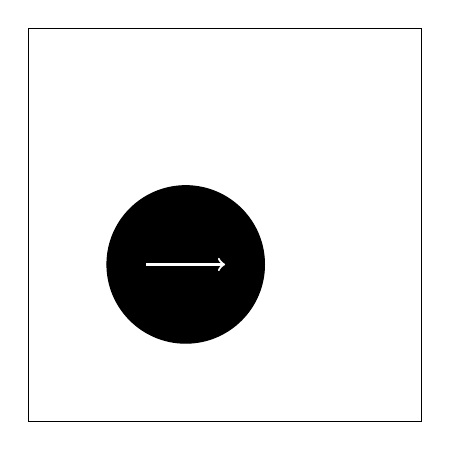
\begin{tikzpicture}
    \draw[](0.0, 0.0) rectangle (5.0, 5.0);
    \draw[fill=black] (2.0, 2.0) circle (1cm);
    \draw[->, draw=white, thick] (1.5, 2.0) -- (2.5, 2.0);
\end{tikzpicture}
\quad
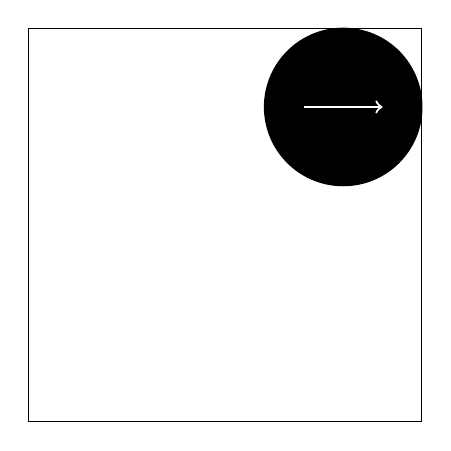
\begin{tikzpicture}
    \draw[](0.0, 0.0) rectangle (5.0, 5.0);
    \draw[fill=black] (4.0, 4.0) circle (1cm);
    \draw[->, draw=white, thick] (3.5, 4.0) -- (4.5, 4.0);
\end{tikzpicture}
    \caption{Example of a data sample. Left hand side is $x$, right hand side is $y$.}
    \label{fig:toy_data_sample}
\end{figure}

Another possibility that is conceptually similar is more in line with other research\cite{kumar2019videoflow}\cite{kipf2019contrastive}. Both Kipf et al. and Kumar et al. make use of similar toy datasets that consist of primary objects and colours and how to manipulate them in various ways. Making use of their dataset(s) would save time and make it more comparable to current research.

\subsubsection*{Realistic real-world dataset idea}
Of course a toy dataset is a good way to get a proof of concept, but it doesn't tell us if our approach will be applicable in any real-world scenario. For that we would need to experiment on more realistic data. That can be done by also constructing a dataset but this time based on real frames form videos. The model would have the same task: learn to predict the causal effect of an intervention from one frame to the next. In the second dataset we could have as a visual clue that is an actual object, such as a red car, that indicates what the intervention would be. If the model learns well, we could then query it things like: "What if the car had been blue?". This would indicate that a different intervention would take place and the outcome image would be transformed differently.

\subsubsection*{Metrics}
What would we define a success in this task? Of course we want a good ELBO but that shouldn't be the goal. If we focus on learning the intervention we want to have some ground truth of $y$ and $t$. Is that different than just the reconstruction loss of $t$ and $y$? We're not necessarily interested in the best reconstruction of $y$ but in the state of the object in the image on which the intervention was applied. We do have a ground truth of the parameters of each object in the image so we could calculate Intersection over Union for example.


\section{Related work: Intersection of generative modelling and causal inference}
In the last few years there have been several papers that have tried to use the power of generative modelling in causal inference to try to learn causal relations from observational studies when a lot of data is available. There also has been research that tried to approach typical deep learning problems from a causal viewpoint in cases where it was beneficial to explicitly take causal relations in the data into account.

\subsubsection*{Causal Effect Inference with Deep Latent-Variable models}
The paper by Louizos et al.\cite{louizos2017causal} serves as a good starting point for research into the use of generative modelling in causal inference. It explores the possibility of measuring the direct effect of one observed variable on another given that there is a shared unobserved confounder by using a proxy variable that has the same confounder. This causal graph is shown in Figure \ref{fig:causal_graph_with_proxy}. Their contribution is doing this task by using Variational Autoencoders\cite{kingma2013auto} to estimate the latent confounder and recover the Individual Treatment Effect, called the CEVAE. They adapt the ELBO equation to accommodate the extra variables in the following way:
\begin{equation}\label{equation:CEVAE_ELBO}
    \begin{split}
-\mathcal{F}(\bx) &= -\mathbb{D}_{KL}[q_\phi(\bz|\bx, \bt, \by) || p(\bz)] + \mathbb{E}_q[\log p_\theta(\bx, \bt|\bz) + \log p_\theta(\by|\bt, \bz)]
    \end{split}    
\end{equation}
We see that the encoder half has been augmented to have three input variables, $\bx, \bt, \by$, and the decoder reconstructs both $\bx$ and $\bt$, and then with $\bt$ it also reconstructs $\by$. That final part in the decoder is where we can manually set the value of $\bt$ to intervene on it.

The paper states that $\bt$ does not have to be binary for their approach to work but it is assumed for simplicity and compatibility with prior benchmarks. They report on how their model does on predicting the ATE and ITE on the Infant Health and Development Program(IHDP) dataset\cite{hill2011bayesian} and introduce a new synthetic dataset based on medical research of the birth weight of twins\cite{almond2005costs}. On both of these dataset the CEVAE does quite well. The dimensionality of the datasets is quite low, so it might be that complexity of these datasets will be exhausted quickly with more powerful models.



\subsubsection*{CausalGAN: Learning Causal Implicit Generative Models with Adversarial Training}
The CausalGAN\cite{kocaoglu2017causalgan}. converts the conditional GAN to a causal GAN, which allows the model to intervene on features instead of conditioning on them. Examples are features such as the person in the image having a moustache. With intervening on that feature instead of conditioning the model can for example generate images of women with moustaches.

As this model is GAN-based, it requires adversarial training. This can generally be considered as a disadvantage as it has unstable training. 

\subsubsection*{A Meta-Transfer Objective for Learning to Disentangle Causal Mechanisms}
Might be relevant, not sure yet.
Disentanglement with causality \cite{Bengio2020A}

\subsubsection*{Causal Confusion in Imitation Learning}
Within imitation learning\cite{torabi2019recent} there is a problem, called causal confusion by de Haan et al.\cite{de2019causal}. This problem arises when there is a feature that is observed by the learner that is highly correlated with the action that the expert takes. However, it is not an indicator that the action should be taken, rather it is an effect that is caused by taking the action. This causes problems for the learner when there is a distributional shift from the training data to the test data, which is always the case in imitation learning. De Haan et al. try to solve this problem by simultaneously learning the causal graph between actions and observations, and which actions lead to a better performance. They show that the learned graph does indeed correspond to the factor that would cause the expert to take a certain action and that the learning agent performs better or equal on benchmarks such as Atari games than the state-of-the-art. 

% We don't explicitly look for the graph by masking latent variables in the decoding, but we do provide a label on what intervention was applied. That is somewhat similar to their expert telling which action it took. We also won't do any actual RL. But Pim doesn't model a prediction from the result of the action, only which action is a 'good' action. Our model can potentially be used for more general queries. Also our interventions aren't discrete.

This research is similar to our approach in the sense that it must learn the effect from an intervention or action by observing visual data. Our approach doesn't involve an explicit learning of the causal connections between each latent variable and the interventions, but instead aims at learning the effect of more complex interventions than the set of discrete actions that is available in a typical reinforcement learning setting. This potentially leads to a model that can predict more complex effects from interventions on a video frame than what the intervention or action is that leads to the highest return.



\subsubsection*{Causal Correct Partial Models for Reinforcement Learning}
Might be relevant, not sure yet.
Causally correct RL: \cite{rezende2020causally}

\subsubsection*{Discovering causal signals in images}
Lopez et al. have investigated the possibility of learning causal signals from visual data \cite{lopez2017discovering}. Their idea was that the presence of certain objects must have been a cause for the presence of other objects in the image. For instance, the presence of a car in an image is a (stochastic) cause for the presence of wheels in the image. 

The paper does look at causal relations within image scenes, but it never models interventions. It only looks if neural net can find correlation between features that are part of objects that have causal relations. It is good to know that a model is capable of distinguishing such features, since we need it for our problem as well.

\subsubsection*{VideoFlow}
The idea of Normalising Flows has also been adapted for video generation, where the model takes a few frames as input and predict the next few frames. This model is called the VideoFlow\cite{kumar2019videoflow}. The basic principle behind the model is that it uses the idea of coupling layers from the Real-NVP to generate frames from the latent vector at that timestep and combines that with an autoregressive prior distribution of the latent vectors, to condition them on all earlier time steps. Because it is a Flow-based model the log-likelihood can be optimised directly and generate frames efficiently compared to a pure autoregressive model.

In a sense it goes beyond what we are trying to achieve because it can predict more than one frame in the future. Though it doesn't distinguish between the role objects and actors play in a scene. It might be a good idea to make use of their architecture for the generation of images/frames from a latent vector.



\bibliography{references.bib}
\bibliographystyle{abbrv}

\end{document}
